\documentclass[../main.tex]{subfiles}
\graphicspath{{\subfix{../}}}
\begin{document}

\chapter{How to Specify IMF Types}
\label{ch:How to Specify IMF Types}
This chapter gives an introduction and step by step guidelines on
how to create an IMF type. Prior understanding of IMF as a framework and language is assumed. Understanding of
reference data libraries is beneficial, but is not required. When explaining how to create IMF types, and advising on
different approaches to take, some examples are provided to make the explanations more concrete. These examples cover
only a few of the possible use cases, and the range of IMF types is likely to be much wider.

\section{The need for IMF Types}
From an engineer's perspective, the following is a valid questioning:
\begin{itemize}
    \item What type of equipment is this? It is a pump.
    \item What type of pump is it? It is a centrifugal pump.
    \item What type of centrifugal pump is is it? It is a two-stage centrifugal pump.
    \item What type of two-stage centrifugal pump is it? It is a flange mounted two-stage centrifugal pump.
\end{itemize}
This questioning could go on, resulting in an ever increasing granularity of typing. As the granularity increases, the level of detail, as well as the precision, increases. But the range of application decreases. In practical applications, there is a need for both high-level IMF types to cover a wide range of use cases, as well as more detailed IMF types for use cases that are more specialised.
The engineer needs to be able to use IMF types to state 'what type of', and for this the IMF type must have a set of attributes that together characterises 'this type of', but a further need is for the IMF type also to be a template holding information which will be re-used every time an instance is created (during modelling). Thus, some attributes are mandatory and hence are part in defining the type, whereas other attributes are optional and offer convenient template information only.


\section{What is an IMF Type?}
IMF types are blueprints for building blocks used to model a facility asset. An IMF type
is a definition from which blocks and terminals are created. 
Basic IMF types are \textit{not} blueprints for complete models, meaning they do not comprise blueprints for, e.g., a breakdown structure, rather they are restricted to templates for one block with terminals (in one aspect). IMF \textit{complex types}, introduced later, allow for more complex patterns.

\subsection{IMF Type and its Role in Information Modelling}
The IMF type provides a pattern with which building blocks are created. The appropriate
IMF type is selected from an IMF type library. The IMF type library is an industry shared resource and thus enables standardisation as well as minimising duplication of work. Prior to being used during modelling, IMF types need to be specified and created such that the IMF type library has sufficient contents.

\begin{figure}[htb]
  \centering
  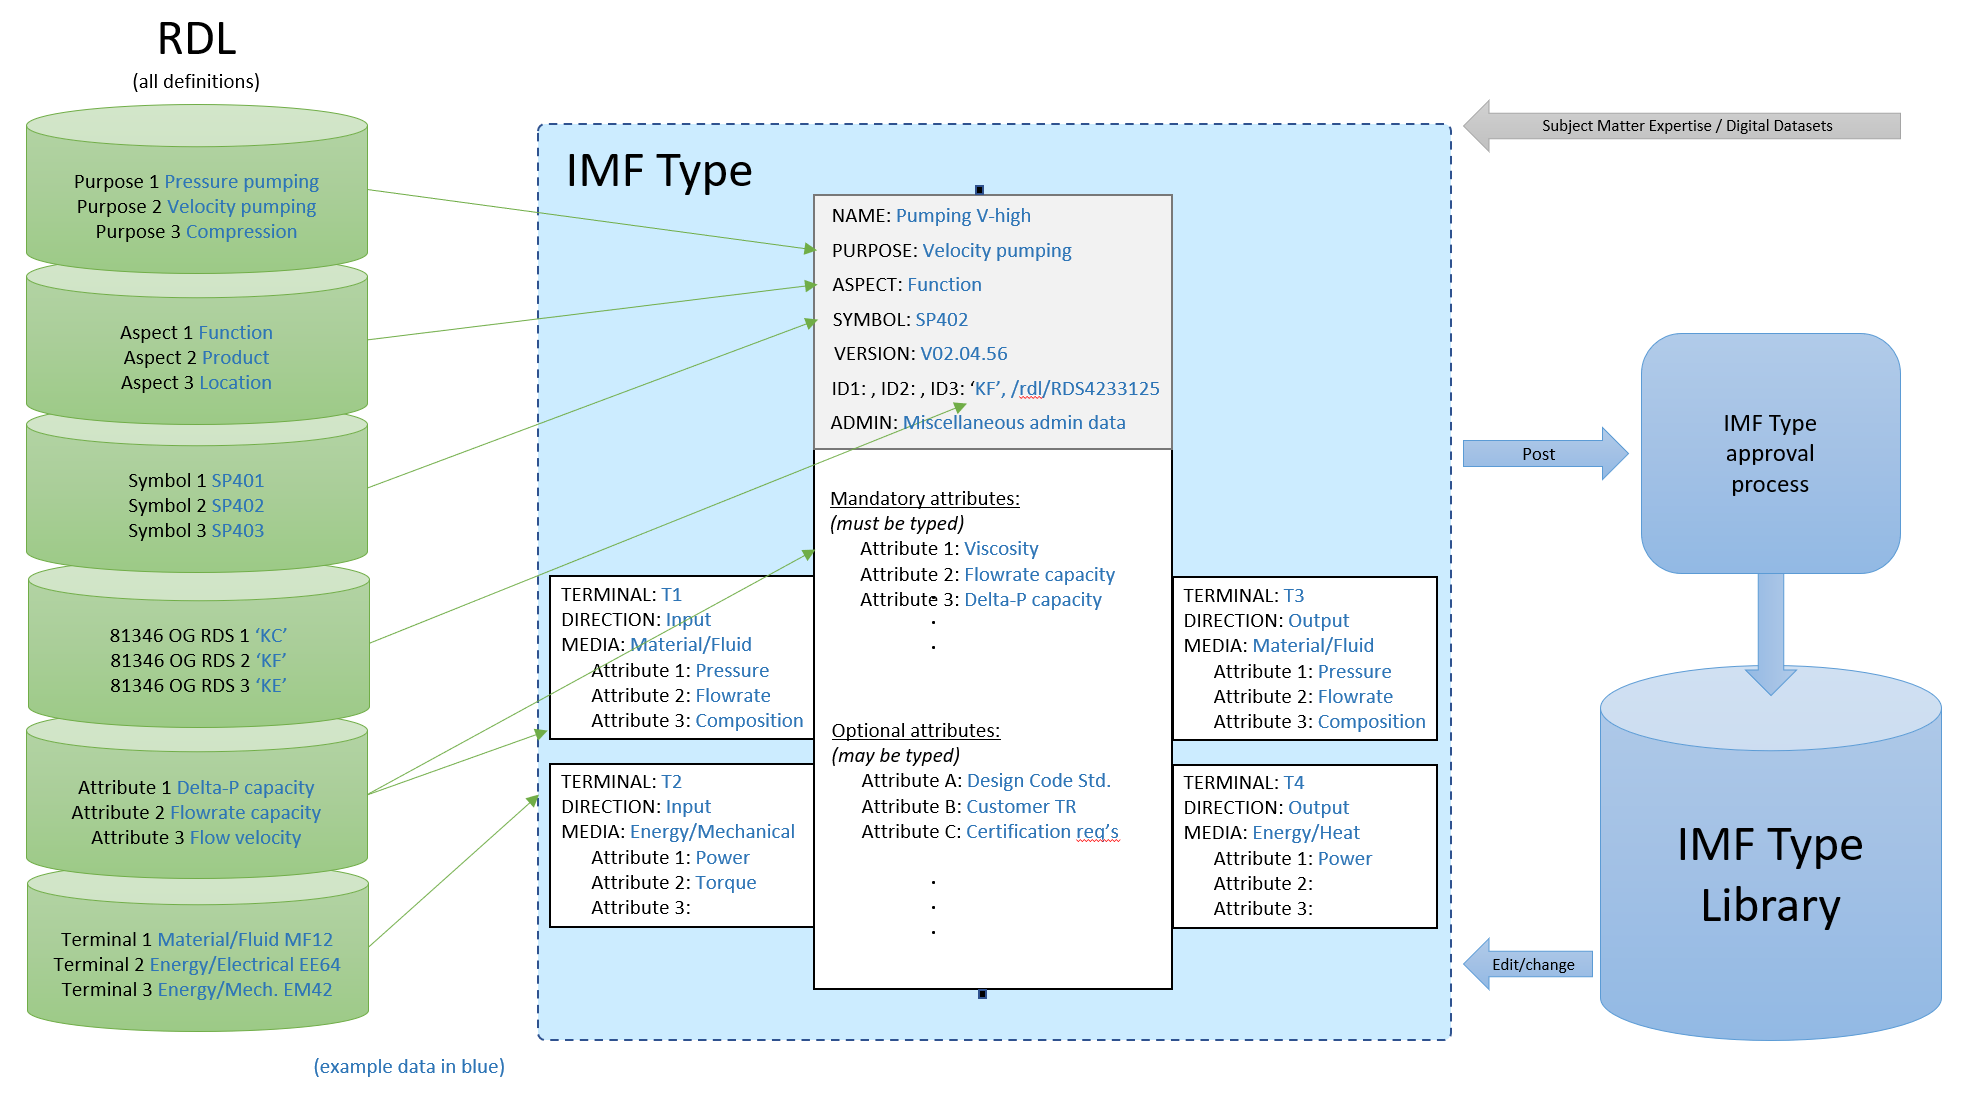
\includegraphics[width=1\textwidth]{img/IMFmanual-img057.png}
  \caption{Creating and using a block with terminals from an IMF type}
  \label{fig:Figure 48}
\end{figure}

\subsection{IMF Type Information Content}
The IMF type contains the information needed to define a building block. There are variants of building blocks, and correspondingly there are variants of IMF types. The information content differs between the variants but adheres to the same basic structure. The properties of an IMF type are sourced from reference data libraries, which are industry shared resources and thus enable standardisation as well as minimising the duplication of work. IMF types are intended to reflect the need of SMEs for building blocks with which they can describe elements of a facility asset. Therefore, the primary input for defining an IMF type is taken from the SME. The means for compiling such domain knowledge could e.g., be datasheets (digital or conventional).


\subsection{IMF Type Aspect of  Information: Function, Product, Location, Installed}
The description of an element of a facility asset differs depending on which aspect of the element is the chosen perspective. Therefore, aspect elements representing each aspect are needed, and consequently,
IMF types representing different aspect are required. The aspects Function, Product, Location, and Installed have been defined in this document. For purposes such as relating to work processes (e.g., procurement), or external data structures (e.g., tagging) creating IMF types in new aspects may be valuable. The IMF language is open in this respect and allows definitions of new aspects.

\subsection{IMF Type Attributes}

An IMF type comprises a range of attributes. These attributes are either mandatory or optional.

\paragraph{Mandatory Attributes} mandatory attributes characterise the IMF type. Data contents for such attributes is a condition for later model validation. To understand which attributes should be mandatory, two guidelines apply:
\begin{enumerate}
\item Identify the attributes that are needed to make the purpose (i.e. the intended activity) of the IMF type as specific as possible.  As an example, an IMF type with purpose Pumping will as a minimum need attributes about Flow and Delta Pressure, as this enables Pumping to be specified at a minimum level.
\item Identify the mandatory attributes of other similar IMF types and make a comparison. There must be a difference in the set of mandatory attributes if the newly created IMF type should be created at all. As an example, if some other IMF type, also with the purpose Pumping, also has the same mandatory attributes about Flow and Delta Pressure, then further differentiation is required. Assuming this example IMF type is about variable speed pumping, then Minimum Speed and Maximum Speed would be appropriate additional mandatory attributes.
\end{enumerate}

\paragraph{Optional Attributes} Optional attributes are \textit{not} essential in characterising the IMF type, but are nevertheless valuable. Typically they represent supplementary information, and can range from being links to reference documents, to being about particular detail data that is of interest when modelling a facility asset. Referring to the Pumping example, an optional attribute could be Design Code or a attribute to hold a reference to a pump curve document.

\paragraph{Additional Attributes} Additional attributes are attributes that are added to individual objects during modelling, but that do not have any relevance to the characteristics of the IMF type from which the object originates. Such attributes can be freely added, as long as they are not in conflict with any of the mandatory attributes. One example, based on the imagined IMF type for Pumping, could be Duty Configuration (with a value of, e.g., `3x50 percent'), which is an attribute which is needed only when the pump is part of a set.

\section{Creating an IMF Type}
\subsection{Target Group}
The primary target group for creating IMF types is the engineering domain SME. To be able to create types, the reference data library needed must be available. This data is likely to be incomplete, which means that
there is a need for close collaboration between the SMEs and the group responsible for creating and maintaining the reference data library, such that needs can be identified and incorporated. This should be supported by a tool and process where SMEs can propose RDL extensions as part of a defined work process.

\subsection{Proactive versus Reactive Workflow}
Maintaining a comprehensive IMF type library requires expert time and resources. Two approaches to this work are valid: proactive and reactive.

\begin{description}
\item[Proactive] creation implies creating IMF types up front, with no specific facility assets in mind, but aiming at creating a useful set of IMF types irrespective of particular facility assets. To scope out what is useful requires understanding of which disciplines come first, of what industry domains have priority, and at what level of granularity will modelling be done during the first stages of facility asset modelling in the industry.
\item[Reactive] creation of IMF types complements the proactive approach in that, as modelling of actual facility
assets progresses, invariably new needs for IMF types will be revealed, and will have to be created in order to enable the modelling to progress.

\end{description}

\subsection{Determining the Aspect of the IMF Type}
When defining an IMF type with a given purpose, it is a prerequisite to understand what the different aspects represent. Only by understanding and choosing the appropriate aspect from which
this IMF type is about to be created, is it possible to choose the applicable attributes and terminals.
\begin{itemize}
  \item \textbf{Function:} In this aspect the need for an essential activity or function is specified, without
        knowledge or decision about how this need may be fulfilled.
  \item \textbf{Product:} In this aspect it is specified how to solve and fulfil a need by means of a component,
        equipment, or assembly.
  \item \textbf{Location:} In this aspect the spatial attributes are defined, including dimensions, relative
        location, and conditions and requirements within the space.
  \item \textbf{Installed:} This aspect is the recorded/documented attributes of a manufactured, delivered or
        installed component, equipment, or assembly.
\end{itemize}

\subsection{Identifying the Purpose of the IMF Type}
At the core of an IMF type definition is its purpose. The purpose is a verb which describes the essence of the IMF type. The value for the purpose is selected from the RDL. One valid purpose which is widely used in examples in this document is Pumping, i.e., `to force an increase flow of-, and/or pressure of a fluid'.
How to select a purpose:
\begin{itemize}
  \item \textbf{Function:} consider what is the essential functionality \emph{needed}, which this particular IMF type shall define the necessary information content for, and choose a purpose which reflects this. Avoid considering a solution to the need, but instead keep the solution space open.

    \emph{Example:} Choose Driving when some sort of mechanical energy needs to be provided for pumping,
                compressing, or other functions that require input of mechanical energy.

  \item \textbf{Product:} consider what is the essential solution \emph{provided}, which this particular IMF type
        shall define the necessary information content for, and choose a purpose which reflects this.

          \textit{Example:} Choose Driving for an electrical motor that provides mechanical rotational energy for, e.g., a pump.


  \item \textbf{Location:} the objective is to define spatial properties, including dimensions and relative location,
        furthermore, to define what conditions are within the space defined, and what requirements apply. Choose Location as purpose when meaning an area, room, or other space that can contain (locate) other entities.

          \textit{Examples:} The spatial properties of an electric motor define its perimeter and relative position. If it
                is not intended to be a location for (contain) other entities, the purpose is the same as in the Product Aspect (Drive). The spatial properties of a cabinet define its perimeter and relative position. It is intended to contain  (locate) entities, therefore the purpose is Locate.

\end{itemize}
Note: With the aspect Location we here refer to the spatial perspective which can be measured along X, Y, Z, e.g., rooms and areas. A different aspect is the Logical Location which is not defined in this document version. It represents a logical ordering, with a breakdown structure that is not identical to the physical breakdown, and where X, Y, Z coordinates are not necessarily relevant. This could be used to define zones having defined activity spaces or states. Examples are Fire Detection, Wifi Coverage, etc.

\begin{itemize}
  \item \textbf{Installed:} consider what is the essential functionality \emph{delivered}, which this particular
        IMF type shall define the necessary information content for, and choose a purpose which reflects this.

          \textit{Example:} Choose Drive for an electrical motor.

\end{itemize}
\subsection{Defining Attributes}
One special attribute of an IMF type is \emph{purpose}. The purpose is a verb which describes the essence of the type, such as Pumping, but alone it does not provide a sufficient specification, which is why mandatory attributes are needed. These attributes are meant
to further specify the purpose, e.g., by specifying capacities and other parameters that answers, `of what', `in what
way', `how much', relating to the purpose. Optional attributes may also be defined as needed, typically to support data that will be repeatedly entered for objects based an IMF type, even if it is not essential information. The qualities of attributes are selected from a reference data library.

\subsection{Assigning the IMF Type to a Class}
An IMF type definition may be a specialisation of a more general IMF type, which again is a
specialisation of a still more general IMF type, and so on, i.e., there is a de-facto hierarchy, even if it is not defined in
advance. By creating a new IMF type on the basis of the more general IMF type, effectively it becomes 
similar to a subclass of the more general IMF type. A hierarchy of types will emerge as more and more
specialised IMF types are created from the more general ones by copying and extending. This hierarchy will provide a
basis for later implementation of a formal class hierarchy. Assigning an IMF type to a class is therefore to state
that it is a specialisation (child) of a more general (parent) IMF type, or a modification (sibling) of some similar
IMF type.

IMF types are selected from, and stored to, the reference data library, governed by a `submit for approval' work
process.

\subsection{Defining Terminals}
Terminals define what the input to and output from a block. The main
properties for a terminal are direction (Input, Output, None/bidirectional) and media (e.g., Process Fluid, Electrical
Current, Information). Additionally, other attributes may allow specifying further details relating to the streaming
medium, such as Volumetric Flow Rate, Electrical Current, Power.

\textbf{Medium Object:} When a higher level of precision is needed, a Medium Object attribute can be specified and
be used to refer to a separate information object which supplies details about the medium composition and state at
this terminal. A medium template defines the structure of a medium object. A medium object specifically for material
is referred to as material object. It may contain a list of chemical components in the material or alternatively a
reference to a defined block in a standard physical properties database such as DIPPR.

Similarly, a medium object specifically for Energy is referred to as an energy object. Such data objects may also be
implemented for Force and Information Media, if needed.

\subsection{IMF Type in the Function Aspect}
In this aspect the \emph{need} for an essential activity or function is specified,
without knowledge or decision about how this need may be fulfilled.

Mandatory attributes are the means for further specifying the purpose, e.g., by specifying capacities and other
parameters that answers, `of what', `in what way', `how much', relating to the purpose.

\emph{Example(s) of function purpose:}
The need for an essential activity or function is specified as the purpose Pumping. The details of what must
        be met by a solution to fulfil this need are provided by mandatory attributes such as Volumetric Flow,
        Delta Pressure, etc.

Optional attributes are for specifying needs that are not directly related to the purpose, and are the means for
stating what must be met by a solution in order to be in compliance with applicable general or overall requirements.

\emph{Example(s) of optional attribute:}
Client requirements such as a specific technical specification which states that there shall be a 50 percent margin on
        all capacity attributes, calculated from the nominal capacity.

Terminals in the Function Aspect specify the stream of a specific medium inputting to or outputting from the activity
or function. Possible media include: Material, Energy, Force, and Information categories, and are selected from the
reference data library.

\emph{Example(s) of terminal:}
An IMF type for an aspect block with purpose Pumping may for instance have a terminal of type
        Input/Material/Fluid/Water.

\begin{figure}[htb]
  \centering
  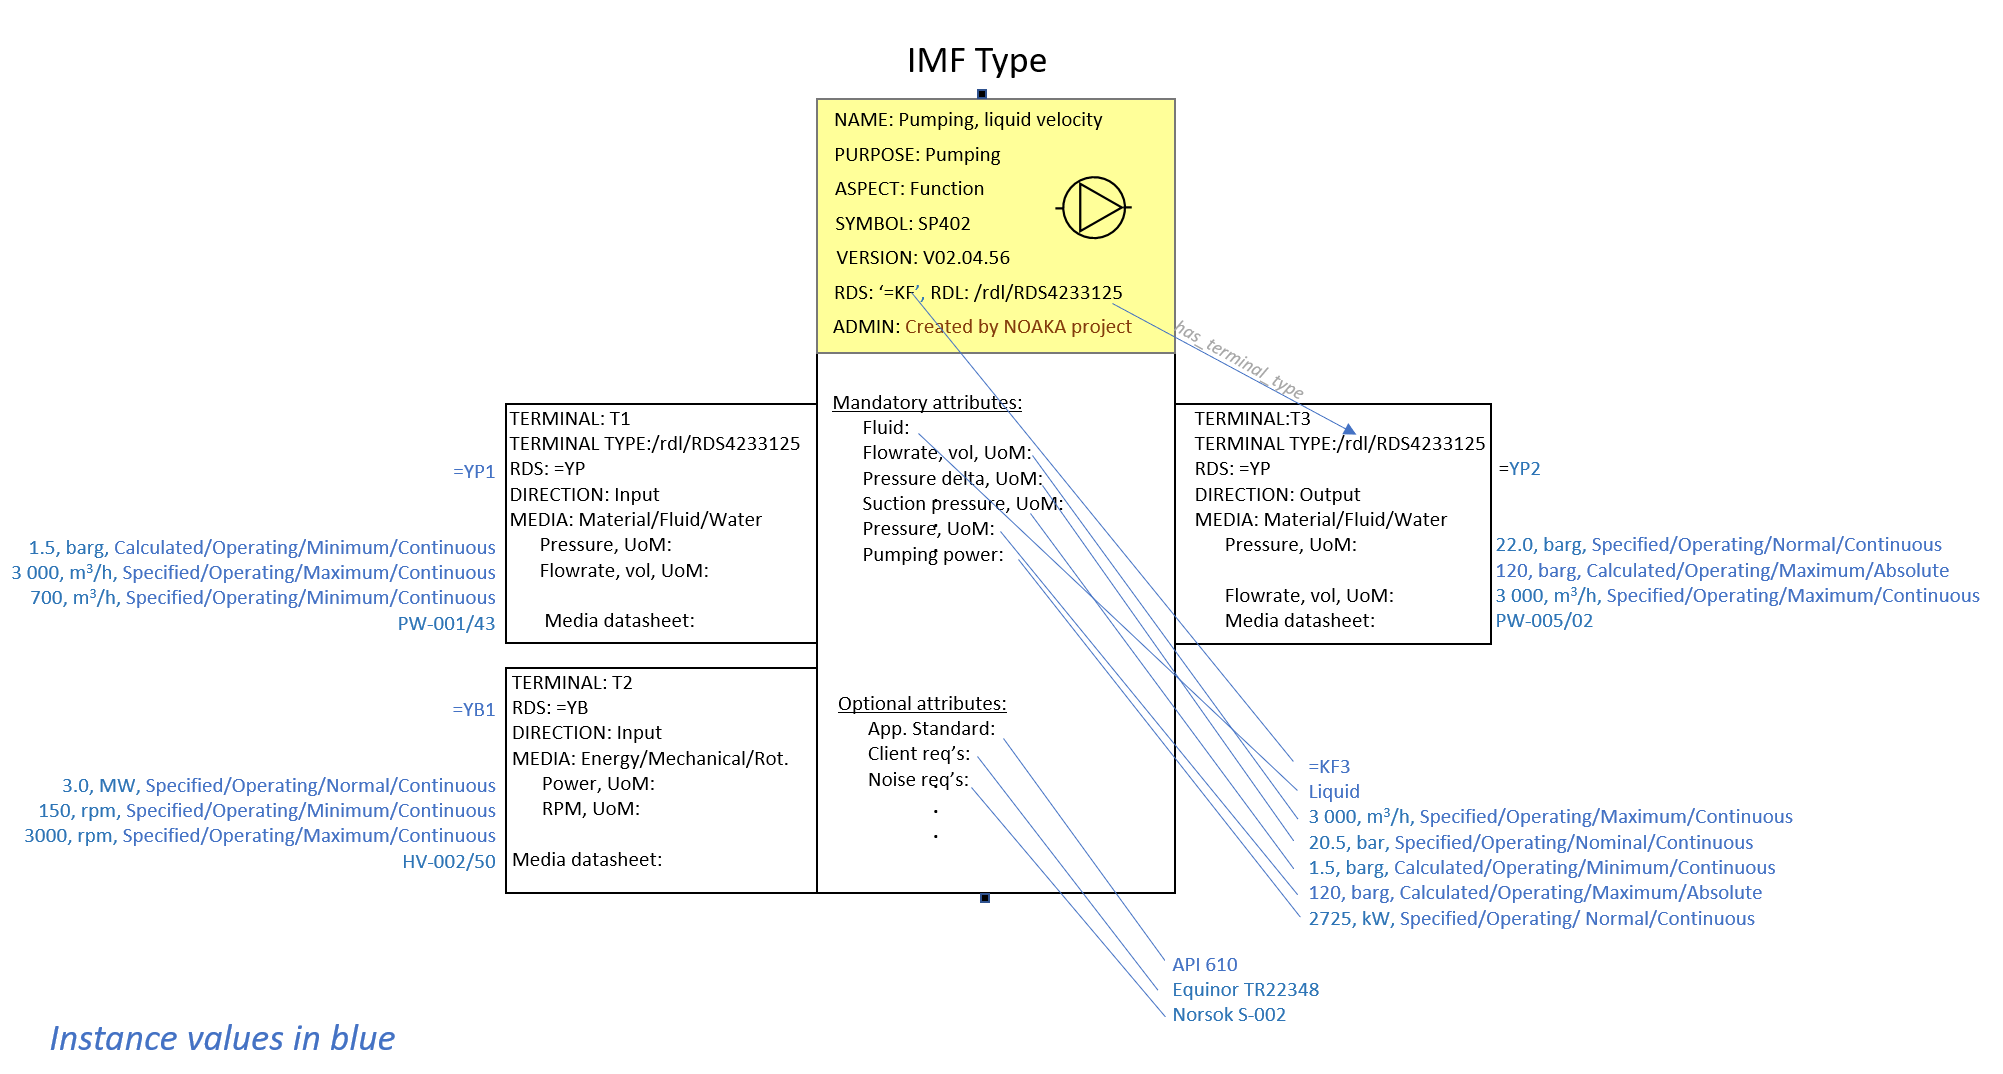
\includegraphics[width=1\textwidth]{img/IMFmanual-img068.png}

  \caption{IMF type example of a Function Aspect.}
  \label{fig:Figure 50}
\end{figure}

\subsection{IMF Type in the Product Aspect}
In this aspect it is specified how to solve and fulfil a need by means of a component,
equipment, or assembly. Mandatory attributes are the means for providing the details of how a solution is specified.

\emph{Example(s) of product purpose:}
The solution is specified as the purpose Pumping. The details of the solution are provided by mandatory
        attributes such as Flow Capacity, Pumping Power, etc.

Optional attributes are for specifying needs that are not directly related to the purpose.

\emph{Example(s) of optional attributes:}
Client requirements such as a specific technical specification which refers to a weight certification
        requirement.

Terminals in the Product Aspect specify the \emph{physical connection} of a specific medium inputting to or
outputting from the activity or function, such as the pipe flange connections or cable termination. Possible media
include: Material, Energy, Force, and Information, and are selected from the reference data library.

\emph{Example(s) of product terminal:}
An IMF type for an aspect block with purpose Pumping may for instance have a terminal of type
        Input/Material/Fluid/Water and a terminal of type Output/Material/Fluid/Water, and would include attributes about flange size, cross section, etc.

\begin{figure}[htb]
  \centering
  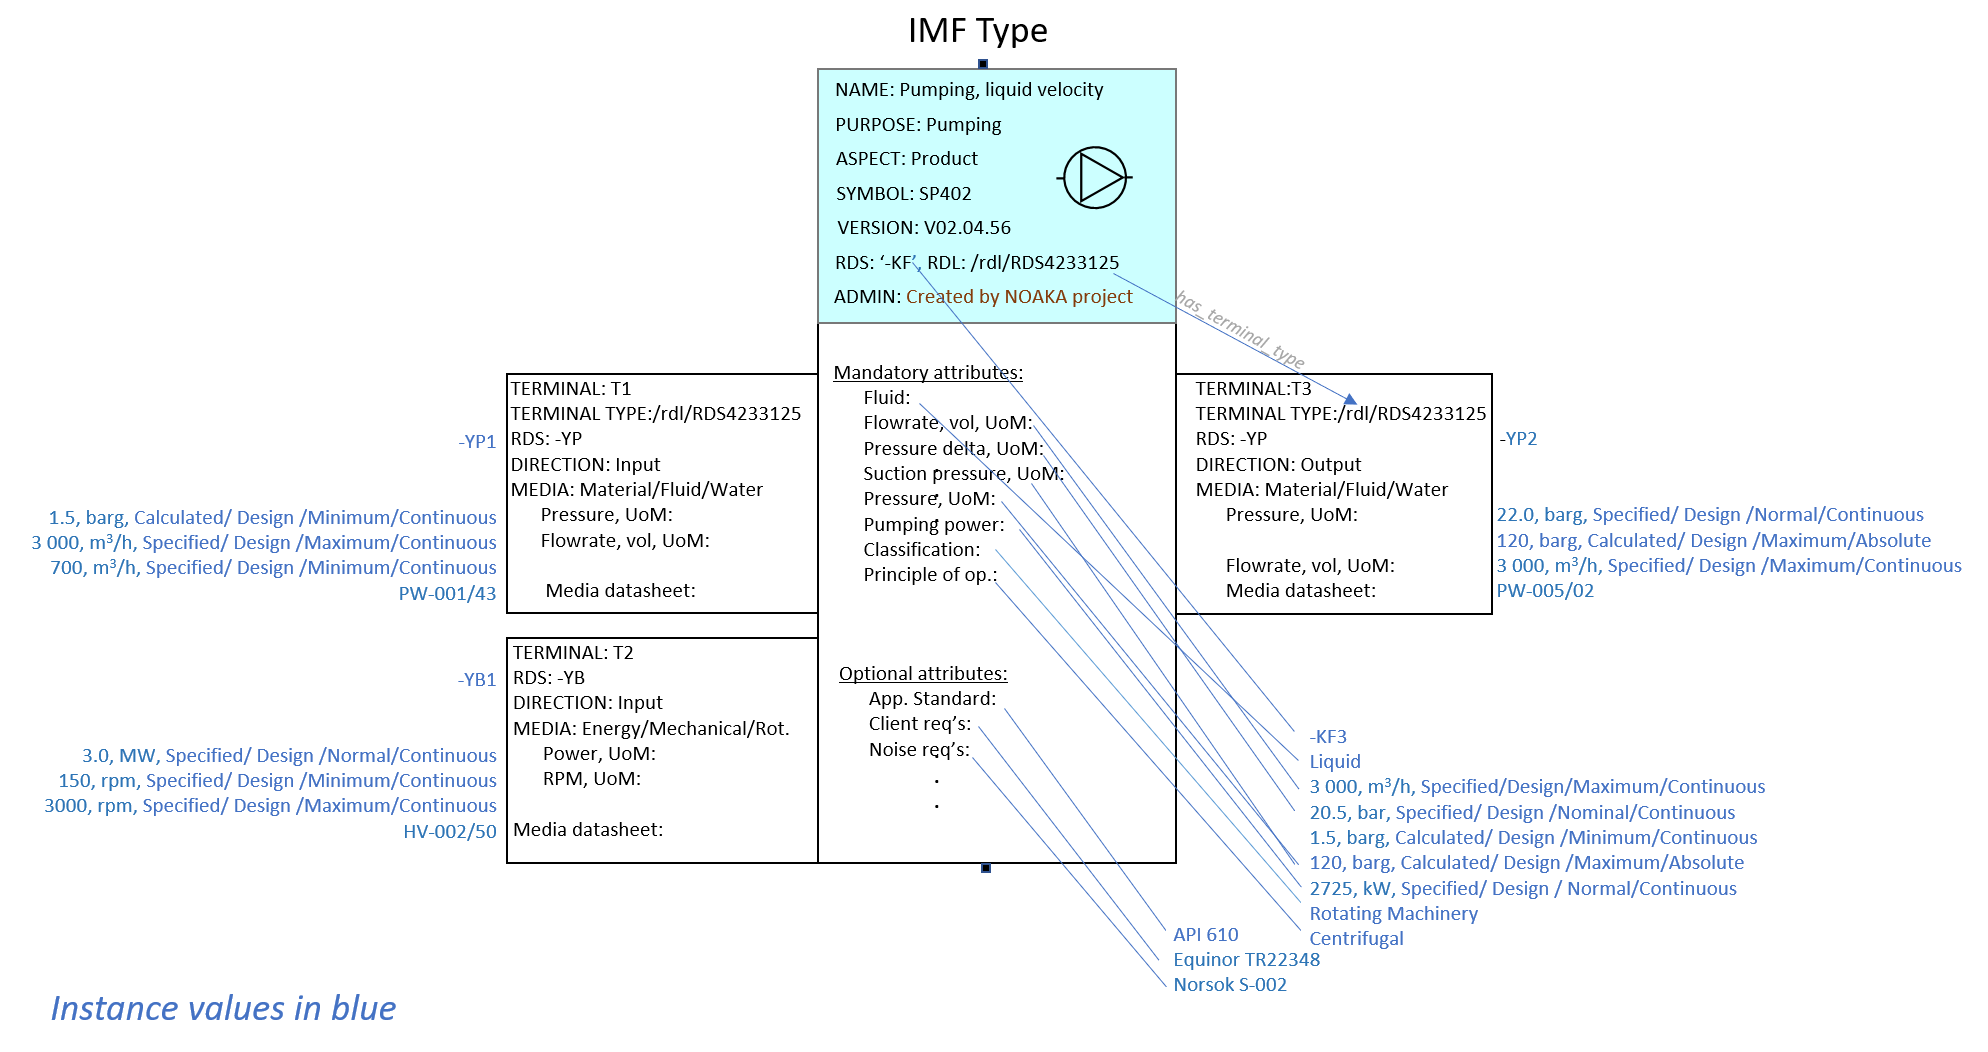
\includegraphics[width=1\textwidth]{img/IMFmanual-img069.png}
  \caption{IMF type example of a Product Aspect.}
  \label{fig:Figure 51}
\end{figure}

\subsection{IMF Type in the Location Aspect}
In the Location Aspect the spatial properties are defined, including dimensions, relative
location, conditions and requirements within the subject area. mandatory attributes are the means for holding this information.

\emph{Example(s) of spatial attributes:}
 A pump has a perimeter, given as Height, Width, Length attributes. It is located in some location, with relative
        position attributes X, Y, Z.
 A processing area has size, given as Height, Width, Length attributes. As a location it is part of some other
        location, with relative position attributes X, Y, Z. Within the space of the area there are specific conditions given
        by area attributes, such as Hazardous Zone Classification.

Optional attributes for area properties specifying conditions and requirements that apply to any component located within this
location (area).

\emph{Example(s) of area properties:}

 Noise requirements that will apply to the emission of noise from any component located in this location.

In the Location Aspect terminals are not used.

\begin{figure}[htb]
  \centering
  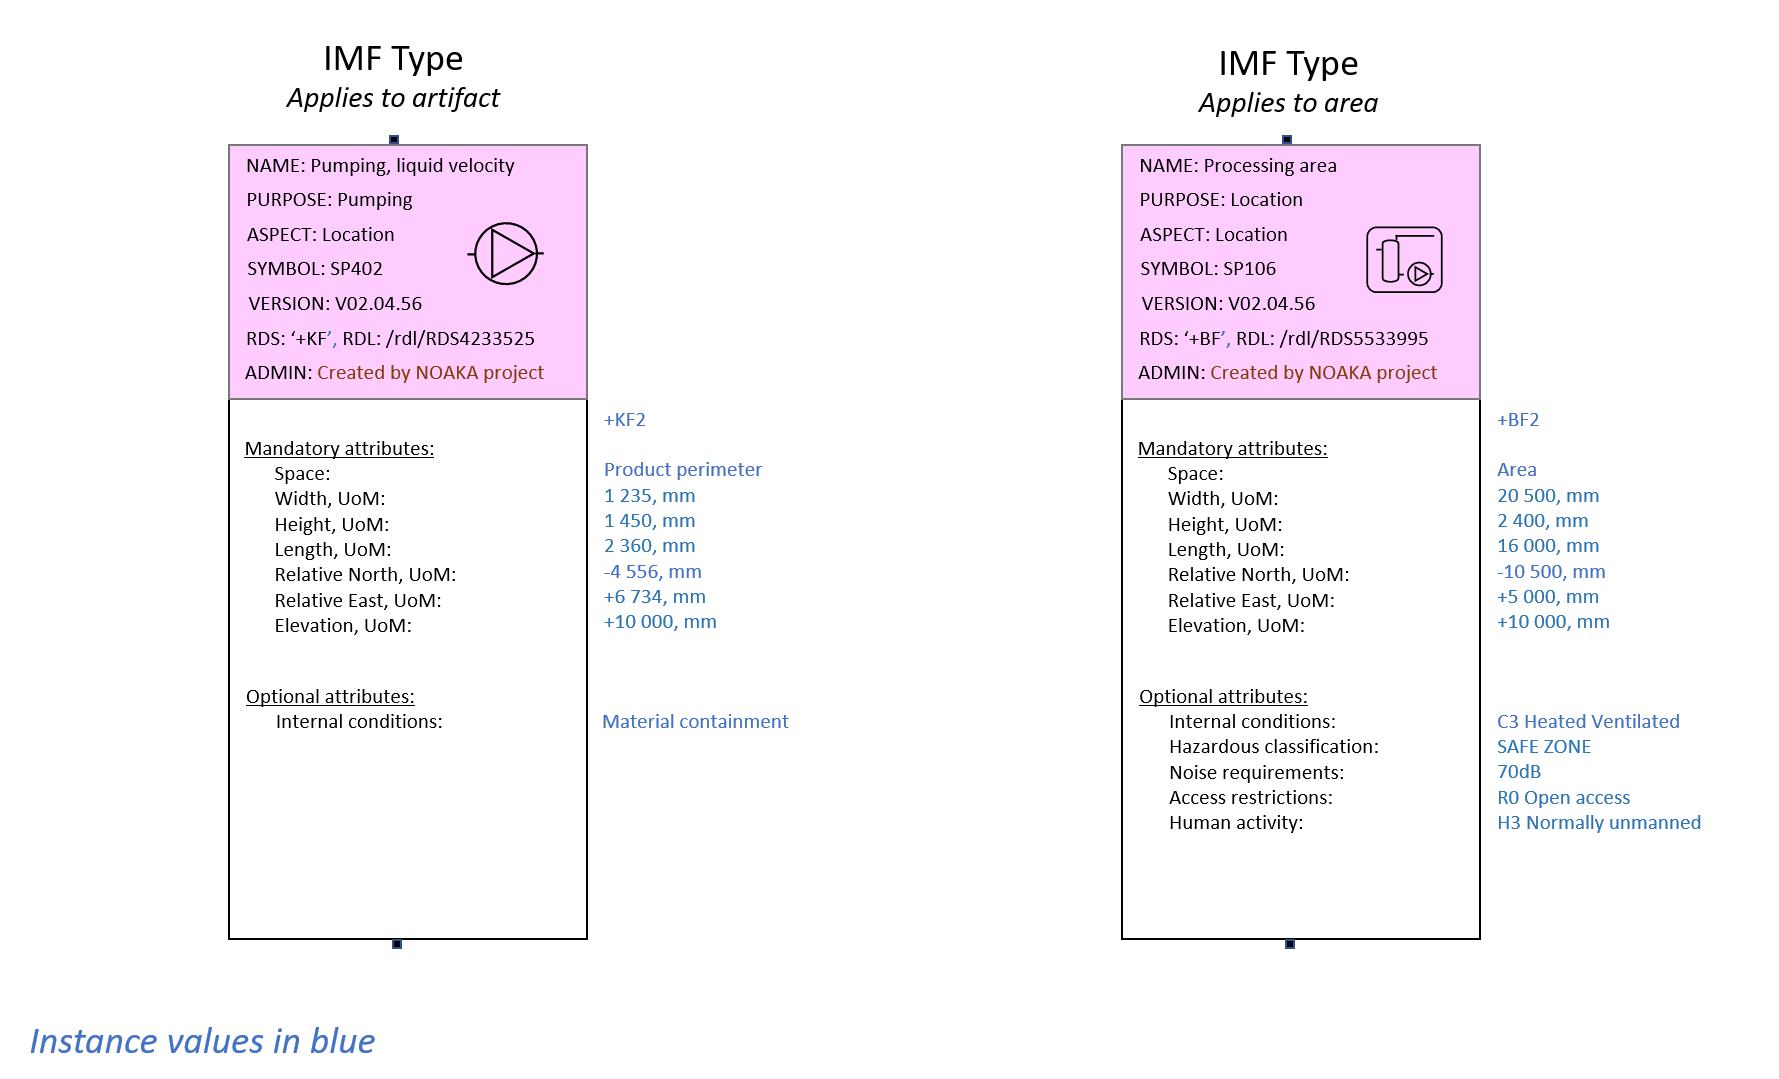
\includegraphics[width=1\textwidth]{img/IMFmanual-img070.png}

  \caption{IMF type example of a Location Aspect.}
  \label{fig:Figure 52}
\end{figure}

\subsection{IMF Type in the Installed Aspect}
This aspect is the manufactured, delivered or installed component, equipment, or assembly,
with its recorded/documented properties. The mandatory attributes are the means for holding this information.

\emph{Example(s) of installed attributes:}
Manufacturers model number.
Reference to a weight certification procedure that has been employed. In the Installed Aspect terminals
        record/document the physical connection of inputs to or outputs from the delivered or installed product.

\begin{figure}[htb]
  \centering
  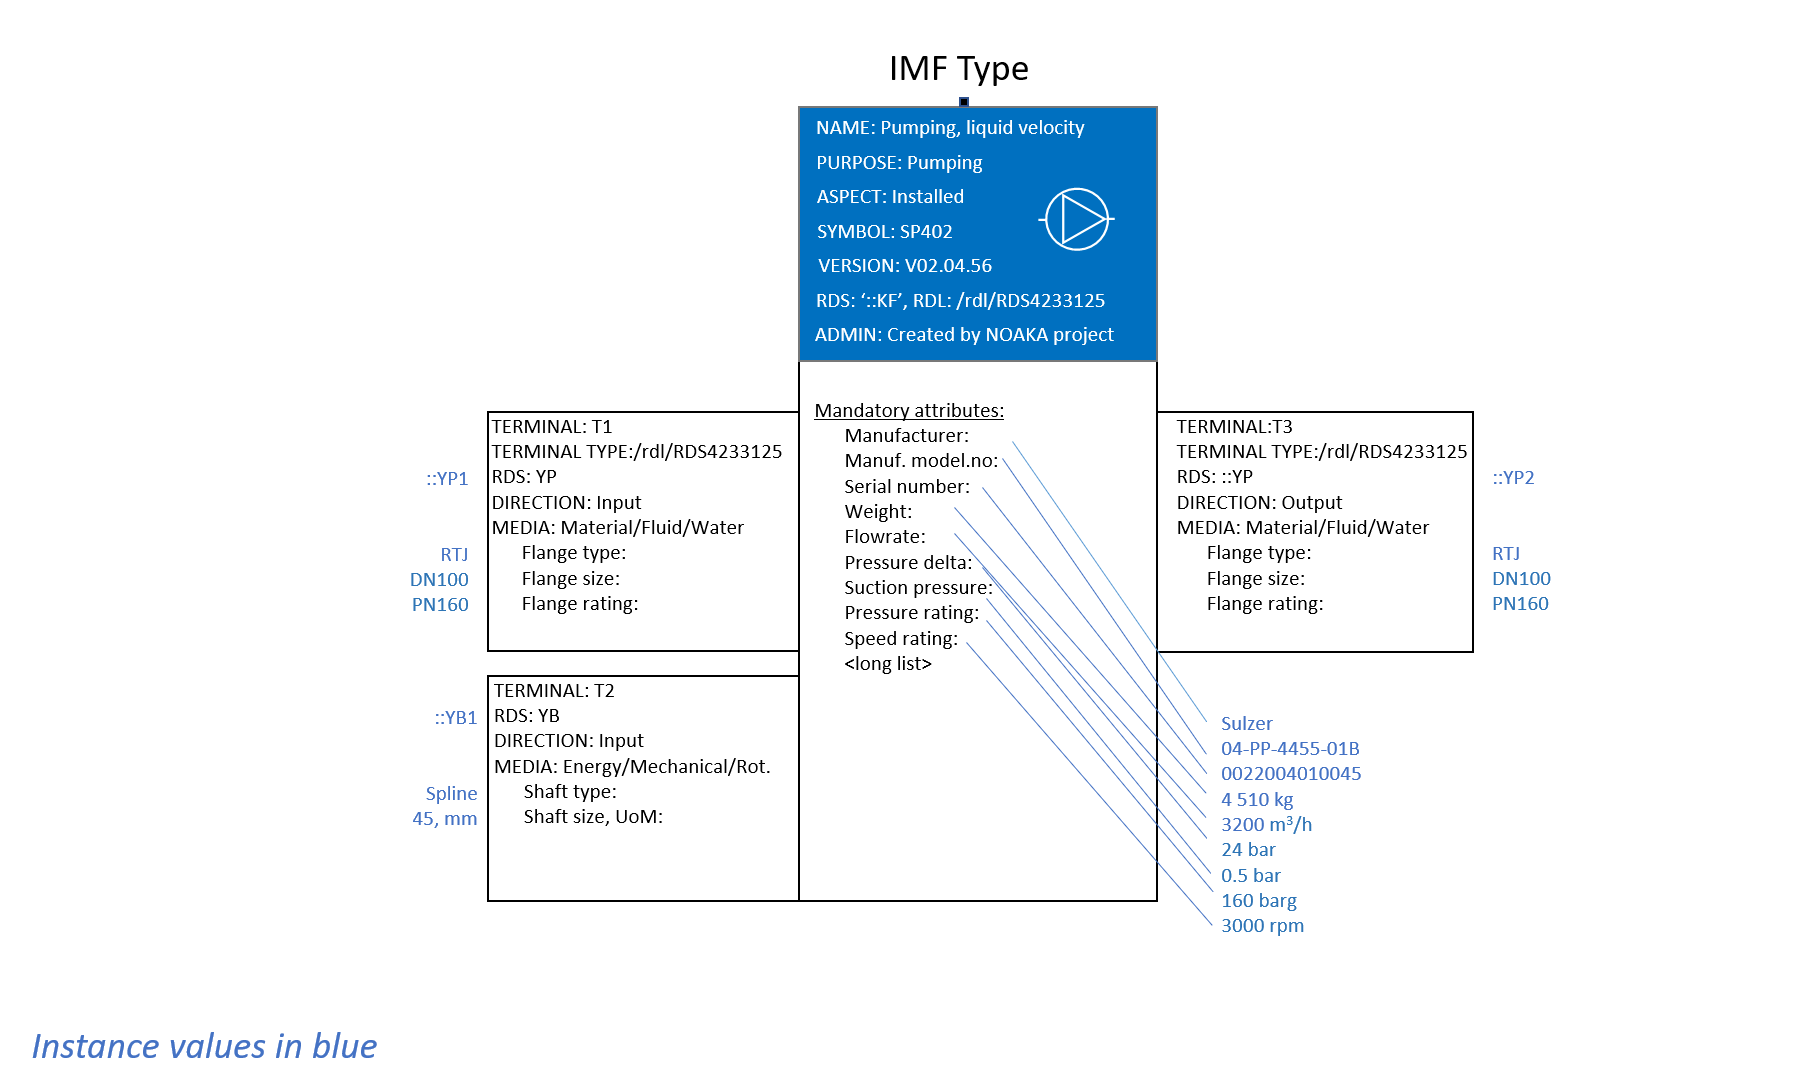
\includegraphics[width=1\textwidth]{img/IMFmanual-img071.png}

  \caption{IMF type example of an Installed Aspect.}
  \label{fig:Figure 53}
\end{figure}

\section{Using Reference Data Libraries}
IMF models contain objects populated with attributes and relations according to the IMF
types. Developing IMF types requires a proper source of standardised definitions of the different concepts an IMF
model needs to utilise. Such sources are often referred to as reference data libraries. Developing IMF types will
be based on the RDL provided by the POSC Caesar Association (PCA).
The reference data is provided in the form
of ontologies represented in the  ontology language OWL.

The PCA RDL contains a comprehensive definition of classes, properties and objects related to industrial
automation systems and life-cycle data for process plants including oil and gas production facilities. Some examples
of such definitions are taxonomies of equipment, process activities and definitions of physical quantities and unit of
measures.

Most of the definitions in the RDL has a reference to the same or similar definition stated in other industrial
standards (where it is applicable) to ensure the possibility to provide different representation of an asset model
according to definitions in different relevant standards.

IMF types will utilise the concepts from the RDL and build any specific IMF type in accordance with the corresponding
concept in the RDL. It will ensure an interoperable IMF asset model provided in the IMF language, which can be
transformed into an RDF data set according the PCA RDL ontologies without loss of information.

\section{[EXPERIMENTAL] Open versus Closed IMF Type}
The default is that an IMF type definition is \textit{open}. That is to say that an object instantiated from it can be freely extended during modelling by additional attributes or by increasing number of terminals, as long as the extension are not in conflict with the type definition.
%Even this limited restriction must be enforced by the user, as there are no mechanisms to prevent it, or invalidate it.
A \emph{closed} IMF type, on the other hand, only allows instantiating objects to set or contain the attributes and terminals that are explicitly permitted by the IMF type. The result is a `stronger' type, with less variance allowed.

\section{[EXPERIMENTAL] What is an IMF Complex Type?}
\label{sec: What is an IMF Complex Type}
Whereas the IMF type provides a template for \textit{one} aspect, and for \textit{one} object, an IMF complex type provides a template for \textit{several} aspects, breakdown structure(s) of \textit{several} objects, and information about how they are interconnected (topology). As such, the IMF complex type can be likened with a small IMF facility asset model.

\subsection{IMF Complex Type and its Role in Information
  Modelling}
  The use case for IMF complex types is to encode design patterns that are frequently employed when building IMF facility asset models. The IMF complex type provides a template for creating instances of such design patterns or even subsystems, and thus support efficient re-use of standardised design patterns.
\subsection{IMF Complex Type Information Content}
To understand what is the information content of an IMF complex type, it is helpful to think of it as a more or less empty model to be later filled in with more details. It comprises breakdown structure(s) of IMF types. It must include this breakdown structure for all the relevant aspects. It may also include information about topology. Further information is optional. Defining more details serve to reduce variance in how a design pattern is implemented, but  will also reduce flexibility during modelling.

\section{[EXPERIMENTAL] Sourcing and inheriting attribute values}
The default is that an attribute of an IMF type, whether it is a mandatory value or an optional value, is without value - because values are assigned to the instance during modelling. This is a very basic functionality which could be enhanced with the following mechanisms:
\begin{itemize}
    \item IMF Type provides a default attribute value:
    \begin{itemize}
        \item The default value is immutable (it contributes to defining the type)
        \item The default value is a typical example value, and can be changed
    \end{itemize}
    \item IMF Type provides constrains to what valid values can be assigned during modelling:
    \begin{itemize}
        \item Equal to value of parent attribute of same attribute type
        \item Larger than value of parent attribute of same attribute type
        \item Less than value of parent attribute of same attribute type
        \item In range of value range of parent attribute of same attribute type
    \end{itemize}

  \item IMF Type provides a mechanism for linking the attribute value to any other attribute value such that it inherits this other value. The specific linking is part of the modelling work. The link may established to any other attribute of the same attribute type within the same IMF model.

  \end{itemize}

\end{document}

 